\titledquestion{Glasspaketet}
De hungriga ungdomarna Asta, Bea och Cesar ska dela på ett glasspaket. Diskussionen uppstår då hur
paketet ska delas rättvist. På kanten finns en markering som de förstår är mitten av paketet (E). Asta
drar då två sträckor utifrån den mittpunkten (AE) samt paketets hörn (BD) (de streckade sträckorna på bilden) och skär sedan av paketet i
skärningspunkten (F) och påstår att hon tagit exakt en tredjedel, den bit som utgörs av fyrhörningen ABHG.
Stämmer det?
\begin{figure}[H]
    \centering
    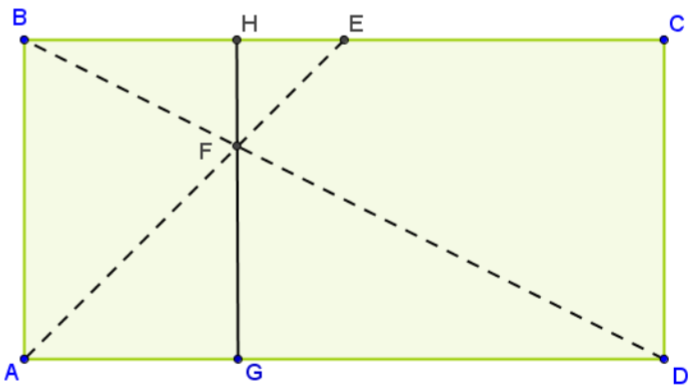
\includegraphics[width=0.5\linewidth]{img/Glasspaket.png}
    \caption{Ett glasspaket.}
\end{figure}